\chapter{Initialization and Termination}
\label{sec:Initialization-and-Termination}

For historical reasons (the 2-dimensional interface was developed first), many
operations have two interfaces, one for two dimensional arrays and the other
for arbitrary dimensional (one- to seven- dimensional, to be more accurate)
arrays. The latter can definitely handle two dimensional arrays as well. The
supported data types are integer,double precision, and double complex. Global
Arrays provide C and Fortran interfaces in the same (mixed-language) program to
the same array objects. The underlying data layout is based on the Fortran
convention.

GA programs require message-passing and Memory Allocator (MA) libraries to
work. Global Arrays is an extension to the message-passing interface.  GA
internally does not allocate local memory from the operating system - all
dynamically allocated local memory comes from MA. We will describe the details
of memory allocation later in this section. 

\section{Message Passing}

The first version of Global Arrays was released in 1994 before robust MPI
implementations became available. At that time, GA worked only with TCGMSG, a
message-passing library that one of the GA authors (Robert Harrison) had
developed before. In 1995, support for MPI was added. At the present time, the
GA distribution still includes the TCGMSG library for backward compatibility
purposes, and because it is small, fast to comple, and provides a minimal
message-passing support required by GA programs. The MPI-compatible version of
GA became the default as of version 5.0. See
\ref{sec:selection-of-the-message-passing-library} for details.

The GA toolkit needs the following functionality from any message-passing
library it runs with:
\begin{itemize}
\item initialization and termination of processes in an SPMD
(single-program-multiple-data) program, 
\item synchronization, 
\item functions that return number of processes and calling process id, 
\item broadcast, 
\item reduction operation for integer and double datatypes, and 
\item a function to abort the running parallel job in case of an error.
\end{itemize}
The message-passing library has to be initialized before the GA library and
terminated after the GA library is terminated.

GA provides two functions \emph{ga\_nnodes} and \emph{ga\_nodeid} that return
the number of processes and the calling process id in a parallel program.
Starting with release 3.0, these functions return the same values as their
message-passing counterparts. In earlier releases of GA on clusters of
workstations, the mapping between GA and message-passing process ids were
nontrivial. In these cases, the \emph{ga\_list\_nodeid} function (now obsolete)
was used to describe the actual mapping.

Although message-passing libraries offer their own barrier (global
synchronization) function, this operation does not wait for completion of the
outstanding GA communication operations. The GA toolkit offers a
\emph{ga\_sync} operation that can be used for synchronization, and it has the
desired effect of waiting for all the outstanding GA operations to complete. 

\section{Memory Allocation}
\label{sub:Memory-Allocation}

GA uses a very limited amount of statically allocated memory to maintain its
data structures and state. Most of the memory is allocated dynamically as
needed, primarily to store data in newly allocated global arrays or as
temporary buffers internally used in some operations, and deallocated when the
operation completes.

There are two flavors of dynamically allocated memory in GA: shared memory and
local memory. Shared memory is a special type of memory allocated from the
operating system (UNIX and Windows) that can be shared between different user
processes (MPI tasks). A process that attaches to a shared memory segment can
access it as if it was local memory. All the data in shared memory is directly
visible to every process that attaches to that segment. On shared memory
systems and clusters of SMP (symmetritc multiprocessor) nodes, shared memory is
used to store global array data and is allocated by the Global Arrays run-time
system called ARMCI. ARMCI uses shared memory to optimize performance and avoid
explicit interprocessor communication within a single shared memory system or
an SMP node. ARMCI allocates shared memory from the operating system in large
segments and then manages memory in each segment in response to the GA
allocation and deallocation calls. Each segment can hold data in many small
global arrays. ARMCI does not return shared memory segments to the operating
system until the program terminates (calls \emph{ga\_terminate}).

On systems that do not offer shared-memory capabilities or when a program is
executed in a serial mode, GA uses local memory to store data in global arrays.

All of the dynamically allocated local memory in GA comes from its companion
library, the Memory Allocator (MA) library. MA allocates and manages local
memory using stack and heap disciplines. Any buffer allocated and deallocated
by a GA operation that needs temporary buffer space comes from the MA stack.
Memory to store data in global arrays comes from heap. MA has additional
features useful for program debugging such as:
\begin{itemize}
\item left and right guards: they are stamps that detect if a memory segment
was overwritten by the application, 
\item named memory segments, and 
\item memory usage statistics for the entire program.
\end{itemize}
Explicit use of MA by the application to manage its non-GA local data
structures is not necessary but encouraged. Because MA is used implicitly by
GA, it has to be initialized before the first global array is allocated.  The
\emph{MA\_init} function requires users to specify memory for heap and stack.
This is because MA:
\begin{itemize}
\item allocates from the operating system only one segment equal in size to the
sum of heap and stack, 
\item manages both allocation schemes using memory coming from opposite ends of
the same segment, and 
\item the boundary between free stack and heap memory is dynamic.
\end{itemize}
It is not important what the stack and heap size argument values are
as long as the aggregate memory consumption by a program does not
exceed their sum at any given time. 

MA is optional for C programs. You can replace GA's internal MA memory handling
with \texttt{malloc()} and \texttt{free()} by using the function
\texttt{GA\_Register\_stack\_memory()}.
\input{replace_ma.tex}

\subsection{Determining the Values of MA Stack and Heap Size}

How can I determine what the values of MA stack and heap size should be? 

The answer to this question depends on the run-time environment of the program
including the availability of shared memory. A part of GA initialization
involves initialization of the ARMCI run-time library.  ARMCI dynamically
determines if the program can use shared memory based on the architecture type
and current configuration of the SMP cluster. For example, on uniprocessor
nodes of the IBM SP shared memory is not used whereas on the SP with SMP nodes
it is. This decision is made at run-time. GA reports the information about the
type of memory used with the function \emph{ga\_uses\_ma()}. This function
returns false when shared memory is used and true when MA is used.

Based on this information, a programmer who cares about the efficient usage of
memory has to consider the amount of memory per single process (MPI task)
needed to store data in global arrays to set the heap size argument value in
ma\_init. The amount of stack space depends on the GA operations used by the
program (for example \emph{ga\_mulmat\_patch} or \emph{ga\_dgemm} need several
MB of buffer space to deliver good performance) but it probably should not be
less than 4MB.  The stack space is only used when a GA operaion is executing
and it is returned to MA when it completes. 

\section{GA Initialization}

The GA library is initialized after a message-passing library and before MA. It
is possible to initialize GA after MA but it is not recommended: GA must first
be initialized to determine if it needs shared or MA memory for storing
distributed array data. There are two alternative functions to initialize GA:

TODO
%\begin{verbatim}
%Fortran  subroutine GA_initialize()
%C        void GA_Initialize()
%C++      void GA::Initialize(int argc, char **argv)
%\end{verbatim}

and

TODO
%\begin{verbatim}
%Fortran  subroutine GA_Initialize_ltd(limit)
%C        void GA_Initialize_ltd(size_t limit) 
%C++      void GA::Initialize(int argc, char **argv, size_t limit)
%\end{verbatim}

The first interface allows GA to consume as much memory as the application
needs to allocate new arrays. The latter call allows the programmer to
establish and enforce a limit within GA on the memory usage.

\emph{Note}: In GA++, there is an additional functionality as follows: 

TODO 
%\begin{verbatim}
%C++      void GA::Initialize(int argc, char *argv[], 
%         unsigned long heapSize, unsigned long stackSize,
%         int type, size_t limit=0) 
%\end{verbatim}

\subsection{Limiting Memory Usage by Global Arrays}

GA offers an optional mechanism that allows a programmer to limit the aggregate
memory consumption used by GA for storing Global Array data. These limits apply
regardless of the type of memory used for storing global array data.They do not
apply to temporary buffer space GA might need to use to execute any particular
operation. The limits are given per process (MPI task) in bytes. If the limit
is set, GA would not allocate more memory in global arrays that would exceed
the specified value - any calls to allocate new arrays that would simply fail
(return false). There are two ways to set the limit:
\begin{enumerate}
\item at initialization time by calling ga\_initialize\_ltd, or 
\item after initialization by calling the function
\end{enumerate}

TODO
%\begin{verbatim}
%Fortran  subroutine ga_set_memory_limit(limit) 
%C        void GA_Set_memory_limit(size_t limit) 
%C++      void GA::GAServices::setMemoryLimit(size_t limit)
%\end{verbatim}

It is encouraged that the user choose the first option, even though the user
can intialize the GA normally and set the memory limit later.

\emph{Example}: Initialization of MA and setting GA memory limits
\begin{verbatim}
call ga_initialize() 
if (ga_uses_ma()) then
   status = ma_init(MT_DBL, stack, heap+global) 
else 
   status = ma_init(mt_dbl,stack,heap) 
call ga_set_memory_limit(ma_sizeof(MT_DBL,global,MT_BYTE)) 
endif 
if(.not. status) ... !we got an error condition here
\end{verbatim}
In this example, depending on the value returned from ga\_uses\_ma(), we either
increase the heap size argument by the amount of memory for global arrays or
set the limit explicitly through ga\_set\_memory\_limit().  When GA memory
comes from MA we do not need to set this limit through the GA interface since
MA enforces its memory limits anyway. In both cases, the maximum amount of
memory acquired from the operating system is capped by the value
\emph{stack+heap+global}. 

\section{Termination}

The normal way to terminate a GA program is to call the function

TODO
%\begin{verbatim}
%Fortran  subroutine ga_terminate() 
%C        void {GA_Terminate() 
%C++      void GA::Terminate()
%\end{verbatim}

The programmer can also abort a running program for example as part
of handling a programmatically detected error condition by calling
the function

TODO
%\begin{verbatim}
%Fortran  subroutine ga_error(message, code)
%C        void GA_Error(char *message, int code)
%C++      void GA::GAServices::error(char *message, int code)
%\end{verbatim}

\section{Creating Arrays - I}

There are three ways to create new arrays:
\begin{enumerate}
\item From scratch, for regular distribution, using

TODO
%\begin{verbatim}
%n-d Fortran  logical function nga_create(type, ndim, 
%                        dims, array_name, chunk, g_a) 
%2-d Fortran  logical function ga_create(type, dim1, 
%
%                        dim2, array\_name, chunk1, chunk2, g\_a) 
%
%{C}           int {NGA\_{}Create}(int type, int ndim, int dims{[}{]}, 
%
%                        char {*}array\_name, int chunk{[}{]}) 
%
%{C++}         GA::GlobalArray{*} GA::GAServices::createGA(int type, 
%
%                        int ndim, int dims{[}{]}, char {*}array\_name, 
%
%                        int chunk{[}{]})
%\end{verbatim}

or for regular distribution, using

TODO
%\begin{verbatim}
%{n-d} {Fortran} logical function {nga\_{}create\_{}irreg}(type, ndim, dims,
%
%                       array\_name, map, nblock, g\_a) 
%
%{2-d} {Fortran} logical function {ga\_{}create\_{}irreg}(type, dim1, dim2,
%
%                       array\_name, map1, nblock1, map2, nblock2, g\_a) 
%
%C           int {NGA\_{}Create\_{}irreg}(int type, int ndim, int dims{[}{]}, 
%
%C++         GA::GlobalArray{*} GA::GAServices::createGA(int type, 
%
%                       int ndim, int dims{[}{]}, char {*}array\_name, 
%
%                       int map{[}{]}, int block{[}{]})
%\end{verbatim}

\item Based on a template (an existing array) with the function

TODO
%\begin{verbatim}
%{Fortran} logical function {ga\_{}duplicate}(g\_a, g\_b, array\_name) 
%
%{C}       int {GA\_{}Duplicate}(int g\_a, char {*}array\_name) 
%
%{C++}     int {GA::GAServices::duplicate}(int g\_a, char {*}array\_name) 
%
%- or - 
%
%{C++}     GA::GlobalArray{*} GA::GAServices::createGA(int g\_a, char
%
%                         {*}array\_name)
%\end{verbatim}

\item Refer to the ``Creating Arrays - II'' section.
\end{enumerate}

In this case, the new array inherits all the properties such as distribution,
datatype and dimensions from the existing array.

With the regular distribution shown in Figure \ref{cap:RegularDistribution},
the programmer can specify block size for none or any dimension. If block size
is not specified the library will create a distribution that attempts to assign
the same number of elements to each processor (for static load balancing
purposes). The actual algorithm used is based on heuristics.

\begin{figure}
\begin{centering}
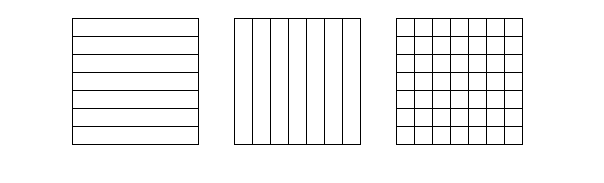
\includegraphics[width=0.9\columnwidth]{distr-1}
\caption{Regular Distribution}
\label{cap:RegularDistribution}
\end{centering}
\end{figure}

With the irregular distribution shown in Figure
\ref{cap:IrregularDistribution}, the programmer specifies distribution points
for every dimension using map array argument. The library creates an array with
the overall distribution that is a Cartesian product of distributions for each
dimension. A specific example is given in the documentation.

\begin{figure}
\begin{centering}
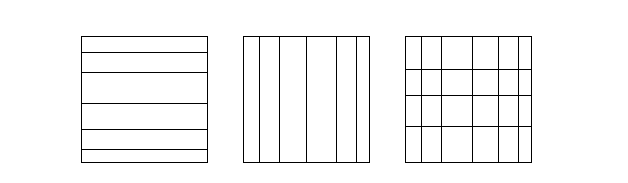
\includegraphics[width=0.9\columnwidth]{distr-2}
\caption{Irregular Distribution}
\label{cap:IrregularDistribution}
\end{centering}
\end{figure}

If an array cannot be created, for example due to memory shortages or an
enforced memory consumption limit, these calls return failure status. Otherwise
an integer handle is returned. This handle represents a global array object in
all operations involving that array. This is the only piece of information the
programmer needs to store for that array. All the properties of the object
(data type, distribution data, name, number of dimensions and values for each
dimension) can be obtained from the library based on the handle at any time,
see Section 7.4. It is not necessary to keep track of this information
explicitly in the application code.

Note that regardless of the distribution type at most one block can be
owned/assigned to a processor. 

\subsection{Creating Arrays with Ghost Cells}

Individual processors ordinarily only hold the portion of global array data
that is represent by the lo and hi index arrays returned by a call to
nga\_distribution or that have been set using the nga\_create\_irreg call.
However, it is possible to create global arrays where this data is padded by a
boundary region of array elements representing portions of the global array
residing on other processors. These boundary regions can be updated with data
from neighboring processors by a call to a single GA function. To create global
arrays with these extra data elements, referred to in the following as ghost
cells, the user needs to call either the functions:

TODO
%\begin{verbatim}
%{n-d} Fortran logical function {nga\_{}create\_{}ghosts}(type, dims, width,
%
%                            array\_name, chunk, g\_a)
%
%{C}           int int {NGA\_{}Create\_{}ghosts}(int type, int ndim, int dims{[}{]},
%
%                            int width{[}{]}, char {*}array\_name, int chunk{[}{]})
%
%{C++}         int GA::GAServices::createGA\_GhostsGA\_Ghosts(int type, int
%
%                            ndim, int dims{[}{]},int width{[}{]}, 
%
%                            char  {*}array\_name, int chunk{[}{]})
%
%{n-d Fortran} logical function {nga\_{}create\_{}ghosts\_{}irreg}(type, dims, width,
%
%                            array\_name, map, block, g\_a) 
%
%{C}           int int {NGA\_{}Create\_{}ghosts\_{}irreg}(int type, int ndim, 
%
%                            int dims{[}{]}, int width{[}{]}, char {*}array\_name,
%
%                            int map{[}{]}, int block{[}{]}) 
%
%{C++}         int GA::GAServices::createGA\_Ghosts(int type, int ndim, 
%
%                            int dims{[}{]}, int width{[}{]}, char {*}array\_name,
%
%                            int map{[}{]}, int block{[}{]}) 
%
%
%\end{verbatim}

These two functions are almost identical to the \texttt{nga\_create} and
\texttt{nga\_create\_irreg} functions described above. The only difference is
the parameter array width. This is used to control the width of the ghost cell
boundaries in each dimension of the global array. Different dimensions can be
padded with different numbers of ghost cells, although it is expected that for
most applications the widths will be the same for all dimensions. If the width
has been set to zero for all dimensions, then these two functions are
completely equivalent to the functions \texttt{nga\_create} and
\texttt{nga\_create\_irreg}. 

To illustrate the use of these functions, an ordinary global array is shown in
Figure \ref{cap:OrdinaryGlobalArray}. The boundaries represent the data that is
held on each processor.

\begin{figure}
\begin{centering}
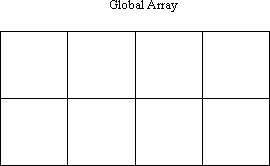
\includegraphics[width=0.9\columnwidth]{ghost003}
\caption{Ordinary Global Array}
\label{cap:OrdinaryGlobalArray}
\end{centering}
\end{figure}

For a global array with ghost cells, the data distribution can be visualized as
shown in Figure \ref{cap:GAwGhostCells}:

\begin{figure}
\begin{centering}
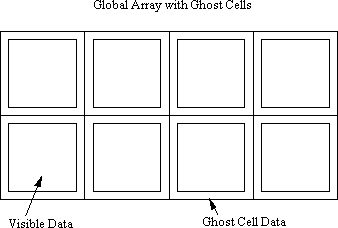
\includegraphics[width=0.9\columnwidth]{ghost006}
\caption{Global Array with Ghost Cells}
\label{cap:GAwGhostCells}
\end{centering}
\end{figure}

Each processor holds ``visible'' data, corresponding to the data held on each
processor of an ordinary global array, and ``ghost cell'' data, corresponding
to neighboring points in the global array that would ordinarily be held on
other processors. This data can be updated in a single call to
\texttt{nga\_update}, described under the collective operations section of the
user documentation. Note that the ghost cell data duplicates some portion of
the data in the visible portion of the global array. The advantage of having
the ghost cells is that this data ordinarily resides on other processors and
can only be retrieved using additional calls. To access the data in the ghost
cells, the user must use the \texttt{nga\_access\_ghosts} function described in
Section 6.1. 

\section{Creating Arrays - II}

As mentioned in the previous section (``Creating arrays - I''), there are 3
ways to create arrays. This section describes method \#3 to create arrays.
Because of the increasingly varied ways that global arrays can be configured, a
set of new interfaces for creating global arrays has been created. This
interface supports all the configurations that were accessible via the old
ga\_create\_XXX calls, as well as new options that can only be accessed using
the new interface. Creating global arrays using the new interface starts by a
call to ga\_create\_handle that returns the user a new global array handle. The
user then calls several ga\_set\_XXX calls to assign properties to this handle.
These properties include the dimension of the array, the data type, the size of
the array, and any other properties that may be relevant. At present, the
available ga\_set\_XXX calls largely reflect properties that are accessible via
the nga\_create\_XXX calls, however, it is anticipated that the range of
properties that can be set using these calls will expand considerably in the
future.  After all the properties have been set, the user calls ga\_allocate on
the array handle and memory is allocated for the array. The array can now be
used in exactly the same way as arrays created using the traditional
ga\_create\_XXX calls. The calls for obtaining a new global array handle are

TODO
%\begin{verbatim}
%{n-d Fortran} integer function {ga\_{}create\_{}handle}() 
%
%{C}           int {GA\_{}Create\_{}handle}()
%\end{verbatim}

Properties of the global arrays can be set using the ga\_set\_XXX
calls. Note that the only required call is to ga\_set\_data. The others
are all optional.

TODO
%\begin{verbatim}
%{n-d Fortran} subroutine {ga\_{}set\_{}data}(g\_a, ndim, dims, type) 
%
%{C}           void {GA\_{}Set\_{}data}(int g\_a, int ndim, int {*}dims, int type)
%\end{verbatim}

The argument \emph{g\_a} is the global array handle, \emph{ndim} is the
dimension of the array, \emph{dims} is an array of \emph{ndim} numbers
containing the dimensions of the array, and \emph{type} is the data type as
defined in either the macdecls.h or mafdecls.h files.  Other options that can
be set using these subroutines are:

TODO
%\begin{verbatim}
%{n-d Fortran} subroutine {ga\_{}set\_{}array\_{}name}(g\_a, array\_name) 
%
%{C}           void {GA\_{}Set\_{}array\_{}name}(int g\_a, char {*}array\_name)
%\end{verbatim}

This subroutine assigns a character string as an array name to the
global array.

TODO
%\begin{verbatim}
%{n-d Fortran} subroutine {ga\_{}set\_{}chunk}(g\_a, chunk) 
%
%C           void {GA\_{}Set\_{}chunk}(int g\_a, int {*}chunk)
%\end{verbatim}

The chunk array contains the minimum size dimensions that should be allocated
to a single processor. If the minimum size is set to -1 for some of the
dimensions, then the minimum size allocation is left to the GA toolkit. The
default setting of the chunk array is -1 along all dimensions.

TODO
%\begin{verbatim}
%{n-d Fortran} subroutine {ga\_{}set\_{}irreg\_{}distr}(g\_a, map, block) 
%
%{C}           void {GA\_{}Set\_{}irreg\_{}distr}(int g\_a, int {*}map, int {*}block)
%\end{verbatim}

The ga\_set\_irreg\_distr subroutine can be used to specify the distribution of
data among processors. The block array contains the processor grid used to lay
out the global array and the map array contains a list of the first indices of
each block along each of the array axes. If the first value in the block array
is M, then the first M values in the map array are the first indices of each
data block along the first axis in the processor grid. Similarly, if the second
value in the block array is N, then the values in the map array from M+1 to M+N
are the first indices of the each data block along the second axis and so on
through the D dimensions of the global array.

TODO
%\begin{verbatim}
%{n-d Fortran} subroutine {ga\_{}set\_{}ghosts}(g\_a, width) 
%
%{C}           void {GA\_{}Set\_{}ghosts}(int g\_a, int {*}width)
%\end{verbatim}

This call can be used to set the ghost cell width along each of the array
dimensions.

TODO
%\begin{verbatim}
%{n-d Fortran} subroutine {ga\_{}set\_{}pgroup}(g\_a, p\_group) 
%
%{C}           void {ga\_{}set\_{}pgroup}(int g\_a, int p\_group)
%\end{verbatim}

This call assigns a processor group to the global array. If no processor group
is assigned to the global array, it is assumed that the global array is created
on the default processor group.

After all the array properties have been set, memory for the global array is
allocated by a call to ga\_allocate. After this call, the global array is ready
for use inside the parallel application.

TODO
%\begin{verbatim}
%{n-d Fortran} logical function {ga\_{}allocate}(g\_a) 
%
%{C}           int {GA\_{}Allocate}(int g\_a)
%\end{verbatim}

This function returns a logical variable that is true if the global array was
successfully allocated and false otherwise. 

\section{Destroying Arrays}

Global arrays can be destroyed by calling the function

TODO
%\begin{verbatim}
%{Fortran} logical {ga\_{}destroy}(g\_a) 
%
%{C}       void {GA\_{}Destroy}(int g\_a) 
%
%{C++}     void GA::GlobalArray::destroy()
%\end{verbatim}

that takes as its argument a handle representing a valid global array.  It is a
fatal error to call ga\_destroy with a handle pointing to an invalid array.

All active global arrays are destroyed implicitly when the user calls
\texttt{ga\_terminate}.
